\newpage
\section{Перечисление альтернированных $k$-танглов}
	\label{section:alternating}

	Для начала заметим, что в любой связной проекции существует только два способа расставить перекрестки альтернированным образом, которые
	мы различать не будем, так как они либо отвечают эквивалентным $k$-танглам, либо отличающимся только зеркальным отражением, которые мы
	тоже отождествляем. Таким образом, все альтернированные танглы мы будем рассматривать как подмножество проекций, содержащее по одному
	представителю из каждого класса эквивалентности по flype-преобразованиям.

	В данной главе мы обсудим генерацию связных простых альтернированных $k$-танглов на основе изложенного в предыдущей алгоритма генерации
	проекций. Однако теперь нам понадобится более сложный способ представления диаграмм, поэтому мы начнем с теоремы, следствиями которой
	будут важные свойства нового представления, описанного в параграфе~\ref{subsection:subtangle-decomposition}.

	\subsection{Теорема о пересекающихся танглах}

		Под словом ``тангл'' ниже будет подразумеваться простую связную диаграмму альтернированного $2$-тангла.

		\begin{theorem}
			\label{theorem:tangle-decomp-th}
			Пусть у нас есть два связных тангла $A$ и $B$, содержащиеся в какой-то простой альтернированной диаграмме
			тангла или зацепления $D$. При этом $A\setminus B\neq\varnothing$, $B\setminus A\neq\varnothing$
			и $A\cap B\neq\varnothing$. Тогда $A\setminus B$, $B\setminus A$, $A\cap B$ и $A\cup B$ --- также связные
			танглы, а $A\cup B$ представим в виде (см. \figureref{figure:tangle-decomp}):

			\begin{figure}[H]
				\centering
				\includegraphics{tangle-decomp-theorem.eps}
				\caption{К Теореме \ref{theorem:tangle-decomp-th}\label{figure:tangle-decomp}}
			\end{figure}
		\end{theorem}
		\begin{proof}
			Обозначим за $a$ количество ребер, ведущих из $A\setminus B$ в остальную часть $D$. Аналогично за $b$ и $c$
			обозначим количество ребер, ведущих в остальную часть $D$ из $B\setminus A$ и из $A\cup B$ соответственно.
			Буквами $d$, $e$ и $f$ обозначим количество ребер между $A\setminus B$ и $A\cup B$, между $B\setminus A$ и
			$A\cup B$ и между $A\setminus B$ и $B\setminus A$ соответственно (см. \figureref{figure:tangle-decomp-proof}).
			Так как $A$ и $B$ --- танглы, то выполняются соотношения:
			\begin{equation}
				\label{equation:a_relation}
				a + c + e + f = 4
			\end{equation}
			\begin{equation}
				\label{equation:b_relation}
				b + c + d + f = 4
			\end{equation}
			Из того, что диаграмма $D$ --- простая, а также из того, что у любого $k$-тангла четное количество ног, следует:
			\begin{equation}
				\label{equation:ab_relation}
				d + e + c \ge 4
			\end{equation}
			\begin{equation}
				\label{equation:all_relation}
				a + b + c \ge 4
			\end{equation}
			\begin{equation}
				\label{equation:amb_relation}
				a + d + f \ge 4
			\end{equation}
			\begin{equation}
				\label{equation:bma_relation}
				b + e + f \ge 4
			\end{equation}
			\begin{figure}[H]
				\centering
				\includegraphics{tangle-decomp-proof.eps}
				\caption{К доказательству Теоремы \ref{theorem:tangle-decomp-th}\label{figure:tangle-decomp-proof}}
			\end{figure}

			Складывая попарно (\ref{equation:a_relation}) и (\ref{equation:b_relation}),
			(\ref{equation:ab_relation}) и (\ref{equation:all_relation}),
			(\ref{equation:amb_relation}) и (\ref{equation:bma_relation}), получаем соответственно:
			\[a + b + d + e + 2c + 2f = 8\]
			\[a + b + d + e + 2c \ge 8\]
			\[a + b + d + e + 2f \ge 8\]
			Отсюда следует, что $c = f = 0$, а все нестрогие неравенства на самом деле являются равенствами. В результате
			получаем систему линейных уравнений на $a$, $b$, $d$ и $e$, единственным решением которой является
			$a = b = d = e = 2$. Завершим доказательство, заметив, что для связности $A\setminus B$, $B\setminus A$ и
			$A\cap B$ достаточно простоты $D$.
		\end{proof}


	\subsection{Разложение на $2$-танглы}
		\label{subsection:subtangle-decomposition}

		Каждая генерируемая диаграмма будет теперь представляться шаблоном --- специального вида проекцией $k$-тангла с таким же
		количеством концов и с меньшим количеством перекрестков, у которого в каждом перекрестке хранится дополнительная информация
		о том, какой из $2$-танглов нужно подставить вместо этого перекрестка, чтобы получить представляемую диаграмму. Похожая
		идея уже ранее использовалась в работе~\cite{SundbergThistlethwaite1998}.
		
		Так же, как и в старом алгоритме, мы будем получать диаграммы, последовательно склеивая их из перекрестков, но теперь разных
		типов перекрестков будет много --- в каждом может быть любой $2$-тангл $T$ любым из $\frac{|D_4|}{|G(T)|}$ способов. Здесь
		$G(T) \subset D_4$ --- група симметрий $2$-тангла $T$.

		Пусть у нас есть $k$-тангл $T$; мы хотим найти единственное разложение $T$ на максимальные $2$-танглы, то есть
		каждому перекрестку $v$ из $T$ сопоставить $2$-тангл $S(v) \subset T$ такой, что:
		\begin{list}{}{}
			\item $v \in S(v)$
			\item $\forall R \subset T$, где $R$ --- $2$-тангл, $v \in R \Rightarrow R \subset S(v)$
			\item $\forall u, u \in S(v) \Leftrightarrow S(u) = S(v)$
		\end{list}
		Заметим, что единственность такого разложения является следствием свойств, выполнения которых мы от него потребовали, а
		существование --- следствием Теоремы \ref{theorem:tangle-decomp-th}, если у исходного тангла имеется как минимум шесть
		концов. В случае же $2$-танглов содержательного (то есть не совпадающего со всем танглом) разложения на $2$-танглы
		может и не существовать. Подобные случаи мы рассмотрим далее.

		\begin{figure}[ht]
			\centering
			\def\pic#1{\raise-14mm\hbox{\includegraphics{tangle-decomp-example-#1.eps}}}
			$$\pic{1} \qquad \Rightarrow \qquad \pic{2}$$
			\caption{Разложение на $2$-танглы}
		\end{figure}

		Заметим, что ни какой flypе не меняет структуру шаблона. Также заметим, что при удалении из шаблона любого пограничного
		перекрестка, не являющегося точкой сочленения или его единственным перекрестком, в результате получается так же корректный
		шаблон какого-либо разложения. Единственное, что осталось сделать для того, чтобы получить весь набор $k$-танглов, имея
		изначально все $2$-танглы с информацией об их группах симметрии, это проверять по ходу склеивания, что у нас по-прежнему
		корректный шаблон, отсекая ``плохие'' ветки и обобщить наш инвариант на такие разложения. Первая задача легко решается
		нахождением минимального разреза, второй посвящен следующий параграф.

	\subsection{Инвариант разложений}

		Введем в каждом перекрестке шаблона $v$ функцию $tangle(v)$ --- неотрицательный номер содержащегося там $2$-тангла. При этом
		потребуем, чтобы у тангла из одного перекрестка был минимально возможный номер. Также введем функцию $orientation(v, e, f)$
		--- ориентацию содержащегося в $v$ $2$-тангла относительно входящего в $v$ ребра $e$ и направления обхода, заданного помеченной
		гранью $f$.

		\begin{algorithm}[ht]
			\caption{root-code-decomp$(P, (v, e, f))$\label{algorithm:root-code-decomp}}
			\algsetup{linenosize=\small, linenodelimiter=.}
			\begin{algorithmic}[1]
				\STATE $A \leftarrow \{\}$
				\STATE $free \leftarrow 2$

				\STATE $Q \leftarrow \{v\}$
				\STATE $number[v] \leftarrow 1$
				\STATE $incoming[v] \leftarrow e$

				\WHILE{$Q \neq \varnothing$}
					\STATE $u \leftarrow head[Q]$
					\STATE $dequeue(Q)$

					\STATE $push(A, tangle(u))$

					\FOR{(для) всех ребер $(u, w) \in P$ в порядке, заданном $f$, начиная с $incoming[u]$}
						\IF{$w$ --- конец диаграммы}
							\STATE $code \leftarrow 0$
						\ELSE
							\IF{$number[w]$ не определен}
								\STATE $number[w] \leftarrow free$
								\STATE $free \leftarrow free + 1$
								\STATE $enqueue(Q, w)$
							\ENDIF
							\STATE $code \leftarrow number[w]$
						\ENDIF

						\STATE $push(A, code)$
					\ENDFOR

					\STATE $push(A, orientation(u, incoming[u], f))$
				\ENDWHILE

				\RETURN $A$
			\end{algorithmic}
		\end{algorithm}

		Аналогично предыдущему определим root-code-decomp($P$, $v$). Заметим теперь, что инвариант, вычисленный в вершине, содержащей
		$2$-тангл из одного перекрестка, всегда будет лексикографиески меньше, чем вычисленный в вершине, содержащей что-то другое.

	\subsection{$2$-танглы}

		Теперь пришло время разобраться с предварительной генерацией $2$-танглов. Проблема с ними состоит в том, что не для каждого
		из них существует нетривиальное разложение. Сформулируем Теорему~\ref{theorem:tangle-sum-th}:

		\begin{theorem}
			\label{theorem:tangle-sum-th}
			Если для какого-то $2$-тангла $T$ не существует корректного разложения на $2$-танглы, то $T$ представим в виде прямой
			суммы двух или более $2$-танглов (см. Рис.~\ref{figure:tangle-sum}).

			\begin{figure}[H]
				\centering
				\includegraphics{tangle-sum.eps}
				\caption{Прямая сумма $T_1, T_2,\cdots, T_s$\label{figure:tangle-sum}}
			\end{figure}
		\end{theorem}
		\begin{proof}
			Если для $T$ не существует разложения на $2$-танглы, то в $T$ есть перекресток $v$ и собственные $2$-подтанглы $A$ и $B$
			такие, что $v \in A$, $v \in B$, $A\setminus B\neq\varnothing$, $B\setminus A\neq\varnothing$ и не существует такого
			собственного подтангла $T$, чтобы он содержал $A$ и $B$. Но по Теореме~\ref{theorem:tangle-decomp-th} $A \cup B$ ---
			$2$-тангл, следовательно $T = A \cup B$.
		\end{proof}
		
		Теорема~\ref{theorem:tangle-sum-th} позволяет однозначно разбить все $2$-танглы на две группы: допускающие разложение в прямую
		сумму и не допускающие. Для второй группы всегда существует корректное разложение на $2$-танглы, поэтому ее можно обрабатывать
		также, как и танглы с большим числом кончов. Разберемся теперь с первой группой.

		В нашем алгоритме танглы первой группы мы будем собирать из их слагаемых. При этом, для поддержания единственности разложения, ни
		одно из слагаемых не должно допускать дальнейшего разложения в прямую сумму в том же направлении. По ходу сборки за этим условием
		следить легко: для каждого $2$-тангла надо запомнить, раскладывается ли он в прямую сумму в этом направлении.

		\begin{figure}[ht]
			\centering
			\includegraphics{one-side-crossings.eps}
			\caption{Перекрестки с одной стороны.\label{figure:one-side-crossings}}
		\end{figure}

		С помощью flype-преобразований можно всегда добиться, чтобы все одиночные перекрестки находились в прямой сумме по одну сторону
		от остальных слагаемых (см.~\figureref{figure:one-side-crossings}) --- варианта их расположения всего два. В силу специфики
		устройства нашего инварианта, мы всегда добавляем к $2$-танглу, содержащему одиночный перекресток на границе только одиночные
		перекрестки, и ничего другого. Поэтому выбирать сторону, с которой будут расположены перекрестки надо только один раз при
		добавлении первого из них. Сделать это можно, сравнив значение инварианта в этих двух конфигурациях. Полностью правила
		сборки прямых сумм приведены в Таблице~\ref{table:sums-rules}.

		\begin{table}[ht]
			\caption{Правила сборки прямых сумм\label{table:sums-rules}}
			\centering
			\begin{tabular}{cm{22mm}l}
				\hline
				1 & \includegraphics{alternating-build-4-case-1.eps} & --- принять \\
				2 & \includegraphics{alternating-build-4-case-2.eps} & --- принять \\
				3 & \includegraphics{alternating-build-4-case-3.eps} & --- сравнить по root-code-decomp \\
				4 & \includegraphics{alternating-build-4-case-4.eps} & --- нарушается положение перекрестков \\
				5 & \includegraphics{alternating-build-4-case-5.eps} & --- нарушается положение перекрестков \\
				6 & \includegraphics{alternating-build-4-case-6.eps} & --- не бывает \\
				7 & \includegraphics{alternating-build-4-case-7.eps} & --- принять \\
				8 & \includegraphics{alternating-build-4-case-8.eps} & --- не бывает \\
				\hline
			\end{tabular}
		\end{table}

		Так как $2$-танглы, вообще говоря, могут обладать симметриями, связанными с поворотами, отражениями или flype-эквивалентностью,
		то согласно \figureref{figure:D4-subgroups} нужно вычислять их группы симметрии, являющиеся одной из 10 подгрупп $D_4$, анализируя
		результаты вычисления инвариантов с разными пометками.

		\begin{figure}
			\centering
			\includegraphics{d4-subgroups.eps}
			\caption{Подгруппы $D_4$.\label{figure:D4-subgroups}}
		\end{figure}

	\subsection{Результаты}

		В Таблице~\ref{table:old-results-table} приведены количества $2$-танглов без учета симметрии (то есть каждый $2$-тангл $T$ нужно
		учесть с весом $\frac{|D_4|}{|G(T)|}$). Результаты согласуются с~\cite{SundbergThistlethwaite1998}.

		\begin{table}[ht]
			\caption{Количество альтернированных $2$-танглов без учета поворотов и отражений.\label{table:old-results-table}}
			\centering
			\begin{tabular}{|r|r|r|r|r|r|r|r|r|r|r|r|}
			\hline
			1 & 2 & 3 &  4 &  5 &  6 &   7 &    8 &    9 &    10 &     11 &     12 \\
			\hline
			1 & 2 & 4 & 10 & 29 & 98 & 372 & 1538 & 6755 & 30996 & 146982 & 715120 \\
			\hline
			\end{tabular}
		\end{table}

		Изображения всех связных простых альтернированных $k$-танглов приведены на \figureref{figure:tangles14} и \figureref{figure:tangles5}.
		В Таблице~\ref{table:alternating-tangles-table} приведены их количества до 12 перекрестков.

		\begin{figure}[ht]
			\centering
			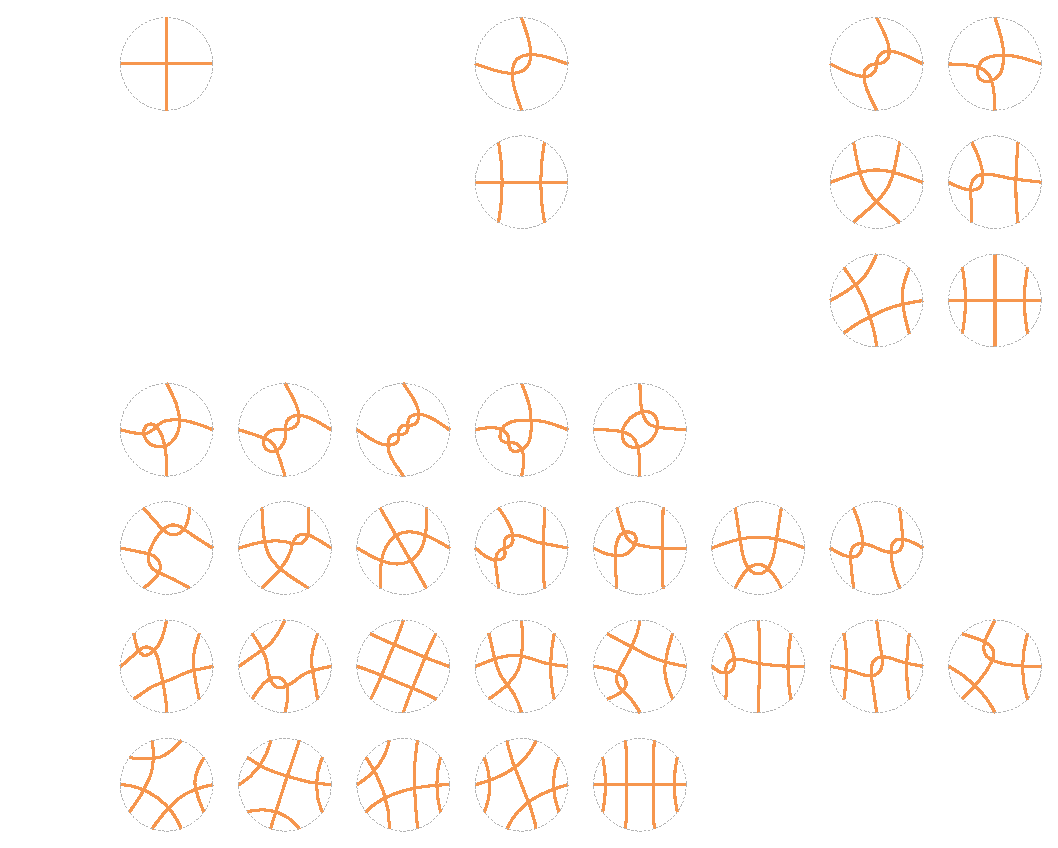
\includegraphics{c/alternating-tangles-1-4.eps}
			\caption{Альтернированные танглы до 4-х перекрестков\label{figure:tangles14}}
		\end{figure}

		\begin{figure}[ht]
			\centering
			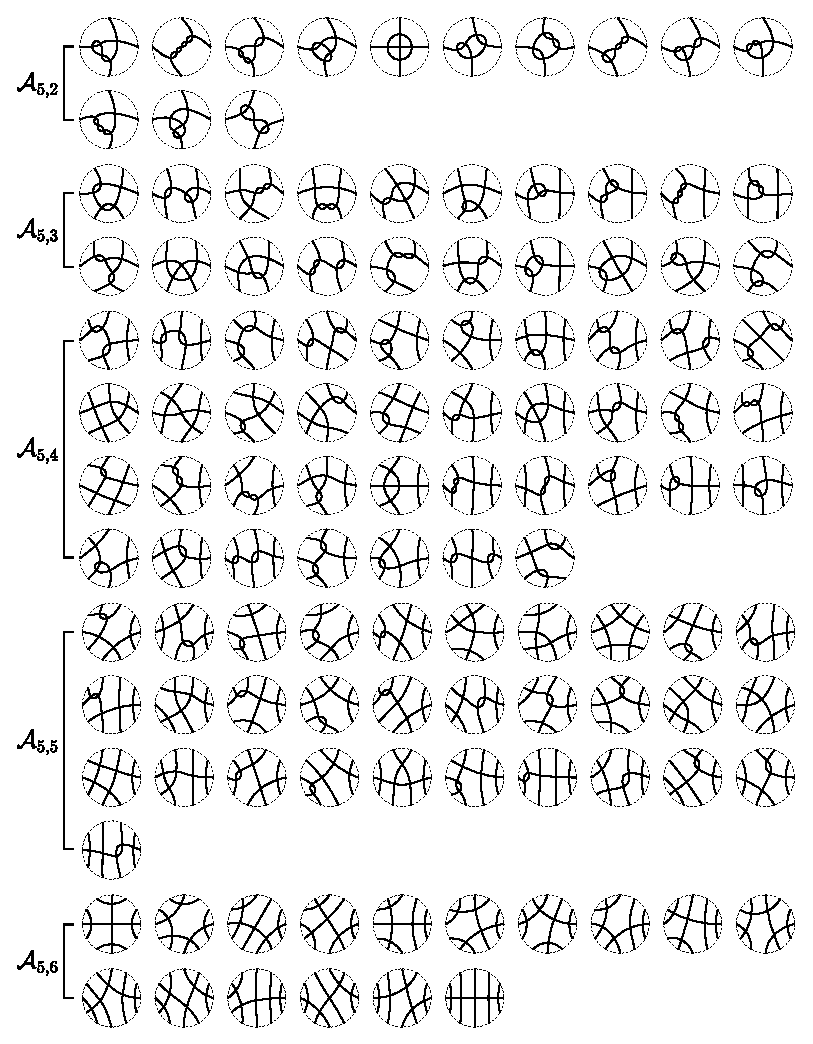
\includegraphics{c/alternating-tangles-5.eps}
			\caption{Альтернированные танглы c 5-ю перекрестками\label{figure:tangles5}}
		\end{figure}

		\begin{landscape}
		\begin{table}[ht]
			\caption{Количество альтернированных $k$-танглов с $n$ перекрестками.\label{table:alternating-tangles-table}}
			\centering
			\begin{tabular}{|c||r|r|r|r|r|r|r|r|r|r|r|r|}
			\hline
			$k$\textbackslash $n$
			    & 1 & 2 & 3 &  4 &   5 &   6 &      7 &       8 &        9 &          10 &           11 &            12 \\
			\hline\hline
			2   & 1 & 1 & 2 &  5 &  13 &  36 &    111 &     373 &   1\,362 &      5\,378 &      22\,807 &      102\,617 \\
			3   & . & 1 & 2 &  7 &  20 &  77 &    276 &  1\,135 &   4\,823 &     21\,734 &     101\,307 &      488\,093 \\
			4   & . & . & 2 &  8 &  37 & 157 &    687 &  3\,052 &  13\,981 &     65\,797 &     317\,506 &   1\,565\,163 \\
			5   & . & . & . &  5 &  31 & 209 & 1\,128 &  5\,986 &  30\,556 &    155\,964 &     795\,918 &   4\,092\,027 \\
			6   & . & . & . &  . &  16 & 161 & 1\,294 &  8\,528 &  51\,475 &    294\,366 &  1\,637\,855 &   8\,979\,493 \\
			7   & . & . & . &  . &   . &  60 &    840 &  8\,206 &  62\,895 &    428\,254 &  2\,702\,902 &  16\,313\,106 \\
			8   & . & . & . &  . &   . &   . &    261 &  4\,702 &  52\,815 &    460\,189 &  3\,475\,551 &  23\,979\,733 \\
			9   & . & . & . &  . &   . &   . &      . &  1\,243 &  26\,753 &    341\,878 &  3\,327\,424 &  27\,625\,056 \\
			10  & . & . & . &  . &   . &   . &      . &       . &   6\,257 &    155\,593 &  2\,221\,544 &  23\,869\,621 \\
			11  & . & . & . &  . &   . &   . &      . &       . &        . &     32\,721 &     916\,595 &  14\,473\,275 \\
			12  & . & . & . &  . &   . &   . &      . &       . &        . &           . &     175\,760 &   5\,464\,661 \\
			13  & . & . & . &  . &   . &   . &      . &       . &        . &           . &            . &      963\,900 \\
			\hline
			все & 1 & 2 & 6 & 25 & 117 & 700 & 4\,597 & 33\,225 & 250\,917 & 1\,961\,874 & 15\,695\,169 & 127\,916\,745 \\
			\hline
			\end{tabular}
		\end{table}
		\end{landscape}
